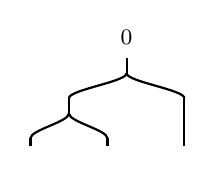
\begin{tikzpicture}[thick, >=stealth, baseline={(current bounding box.center)}, scale=0.850]
\begin{scope}[shift={(0.000,0.000)}, scale=1.000]
  \draw (-1.150,-0.120) .. controls (-1.150,-0.080) and (-1.150,-0.040) .. (-1.150,0.000);
  \draw (0.000,-0.120) .. controls (0.000,-0.080) and (0.000,-0.040) .. (0.000,0.000);
  \draw (1.150,-0.120) .. controls (1.150,-0.080) and (1.150,-0.040) .. (1.150,0.000);
  \draw (1.150,0.000) .. controls (1.150,0.200) and (1.150,0.400) .. (1.150,0.600);
  \draw (-0.575,0.370) .. controls (-0.575,0.447) and (-0.575,0.523) .. (-0.575,0.600);
  \draw (0.287,0.970) .. controls (0.287,1.047) and (0.287,1.123) .. (0.287,1.200);
  \draw (-1.150,0.000) .. controls (-1.150,0.123) and (-0.575,0.247) .. (-0.575,0.370);
  \draw (0.000,0.000) .. controls (0.000,0.123) and (-0.575,0.247) .. (-0.575,0.370);
  \draw (-0.575,0.600) .. controls (-0.575,0.723) and (0.287,0.847) .. (0.287,0.970);
  \draw (1.150,0.600) .. controls (1.150,0.723) and (0.287,0.847) .. (0.287,0.970);
\end{scope}
\begin{scope}[shift={(0.000,0.000)}, scale=1.000]
\end{scope}
\begin{scope}[shift={(0.000,0.000)}, scale=1.000, every node/.style={inner sep=1pt, font=\footnotesize}]
  \node[anchor=west, fill=white, inner sep=0.8pt] at (-0.455,0.485) {\ftreeinner};
  \node[anchor=north] at (-1.150,-0.200) {\ftreelegA};
  \node[anchor=north] at (0.000,-0.200) {\ftreelegB};
  \node[anchor=north] at (1.150,-0.200) {\ftreelegC};
  \node[anchor=south] at (0.287,1.340) {0};
\end{scope}
\end{tikzpicture}
